\documentclass[11pt]{article}
\usepackage{amsmath}
\usepackage{amssymb}
\usepackage{hyperref}
\usepackage{graphicx}
\usepackage{color}
\usepackage{cite}
\usepackage{framed}
\usepackage[margin=0.95in]{geometry}
\usepackage[parfill]{parskip}
\setlength{\parindent}{0pt}
\begin{document}

\title{Study of Charge and Lattice Dynamics in Quantum Materials}
\author{Xunyang Hong}
\date{}
\maketitle





\begin{abstract}
This proposal presents a focused study on electron-phonon coupling (EPC) in quantum matter using resonant inelastic X-ray scattering (RIXS) across three projects. \textbf{(1)} The first project aims to investigate the interaction between charge order and EPC in cuprate superconductors, particularly {La$_{1.8-x}$Eu$_{0.2}$Sr$_x$CuO$_{4}$}, to understand interplay between phonons and charge order excitations. \textbf{(2)} The second project explores the electron-phonon dynamics in SrTiO$_{3}$ and KTaO$_{3}$, examining the reversed isotope effect and orientation-dependent superconductivity, respectively, by measurement of the EPC via RIXS. \textbf{(3)} Finally, the study extends to sapphire to measure its EPC, aiming to facilitate sub-MeV dark matter detection.
Furthermore, numerical technique will also be developed to facilitate the simulation of RIXS spectra, and the extraction of EPC. These projects collectively aim to deepen our understanding of electron-phonon interactions and their implications in superconductivity and dark matter research.
\end{abstract}

\section{Objectives of the project}
% \textit{\textbf{Instruction}: Please present the rationale for your project based on the current state of knowledge in the respective field, list the {\color{cyan}general research question} and the {\color{cyan}specific objectives}, mention the {\color{cyan}research methods}, and briefly discuss the {\color{cyan}expected results} and their implications for your field}

% simulation in MS thesis, and expand the theory?
% polaron in STO. 

\paragraph{Research question and objectives}
Electron-phonon coupling (EPC) is fundamental to the understanding of many phenomena in condensed matter physics, such as superconductivity\cite{bardeen_theory_1957,cuk_review_2005} and charge order\cite{arpaia_charge_2021,comin_resonant_2016,tranquada_spins_2013}.
%and even dark matter detection\cite{griffin_directional_2018}. 
In conventional superconductors that obey Bardeen-Cooper-Schrieffer (BCS) theory, phonon is believed to mediate the superconductivity\cite{bardeen_theory_1957}. 
Thus understanding EPC is crucial in conventional superconductivity. 
However, even in high-temperature superconductors, despite the lack of a fully understood mechanism, EPC is still playing an important role in many unconventional superconducting systems: \textbf{(1)} static and dynamical charge order observed in cuprate superconductors is hypothesized to interact with phonons, possibly stemming from special features in electron-phonon interaction\cite{lin_strongly_2020, wang_charge_2021, huang_quantum_2021, miao_incommensurate_2018,tacon_inelastic_2014,li_multiorbital_2020,li_multiorbital_2020,chaix_dispersive_2017,braicovich_determining_2020,huang_quantum_2021}; 
\textbf{(2)} Strong EPC gives rise to a novel excitation, polaron, in $\mathrm{SrTiO_3}$ and $\mathrm{KTaO_3}$, leading to intriguing phenomena\cite{swartz_polaronic_2018,chen_orientation-dependent_2023}. 

However, measuring the EPC is very challenging. 
It is indeed difficult to find techniques that are directly sensitive to this interaction. Most of the time, it can only be extracted through very indirect methods (i.e. measuring the ``kink" of the electron dispersion in ARPES spectra).

Thanks to the recent technological advancements in resonant inelastic x-ray scattering (RIXS), it is now possible to achieve an energy resolution sufficient to measure phonon bands. 
More importantly, it can be shown that the RIXS cross section for phonons is directly related to the EPC\cite{ament_determining_2011, devereaux_directly_2016}. 
At present, however, the exact value of EPC can only be extracted from the experimental spectra in a few simple systems, with stringent assumptions and approximation\cite{braicovich_determining_2020,vale_high-resolution_2019}. 
Therefore, there is an urgent need for further numerical technique to extend the RIXS model to a broader range of superconducting materials, thereby enabling the extraction of EPC in these systems. 

In the course of my PhD. research, I propose three projects to study electron-phonon interaction in different systems, employing the state-of-the-art high-resolution resonant inelastic x-ray scattering (RIXS) technique\cite{ament_resonant_2011,zhou_i21_2022}. 
My aim is not only to perform RIXS experiments to investigate EPC, but also to develop the theoretical and numerical methods for simulating RIXS spectra beyond the model proposed in Ref.\cite{ament_determining_2011}, to better assisting extracting EPC in various quantum systems.
\begin{figure}[!t]
    \centering
    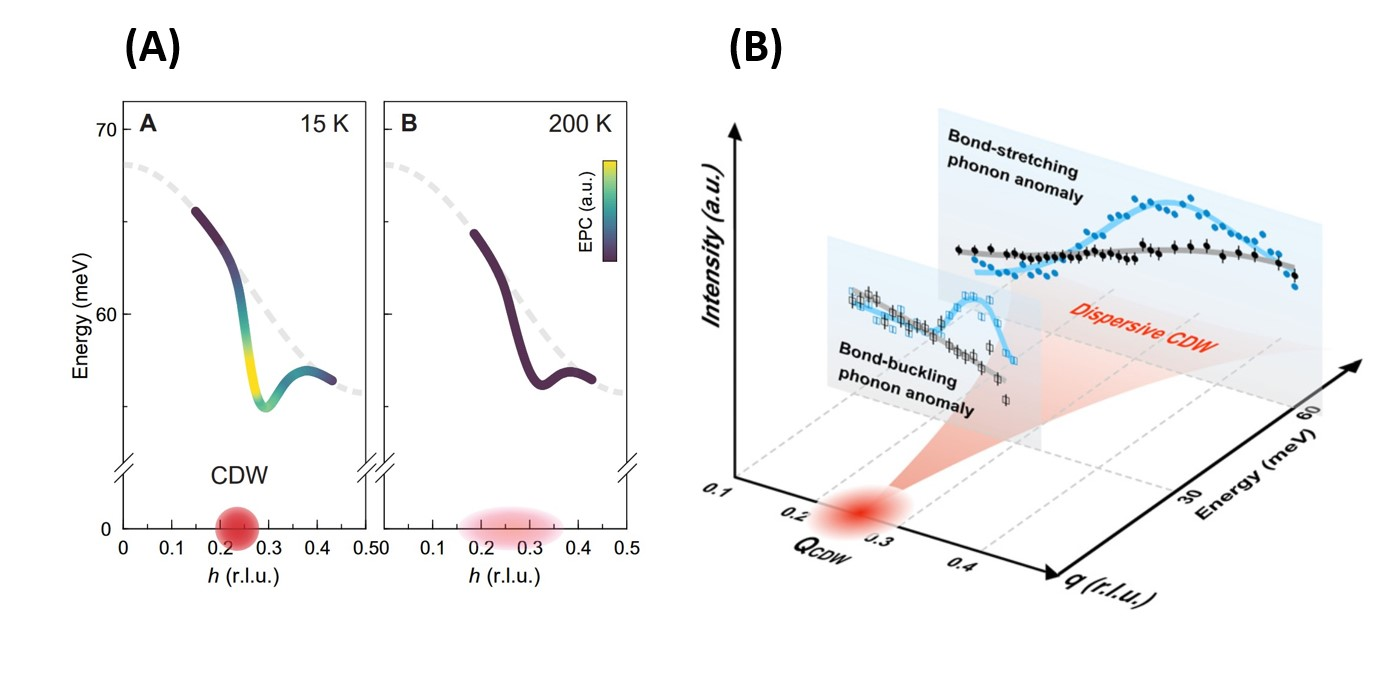
\includegraphics[width=0.8\textwidth]{figures/new_first_figure.jpg}
    \caption{\textbf{(A)}: Dispersion of bond-stretching phonon in $\mathrm{La_{1.675}Eu_{0.2}Sr_{0.125}CuO_{4}}$. Phonon softening and Enhancement in electron-phonon coupling (EPC) near charge order (CDW) observed in  through RIXS at Cu-L edge; The color in the curve indicates the extracted EPC (from Ref.\cite{wang_charge_2021}); \textbf{(B)} A sketch of phonon intensity as a function of momentum. Phonon intensity anomaly near charge order (CDW) observed in $\mathrm{Bi_2Sr_2LaCuO_{6+\delta}}$ through RIXS.  (from Ref.\cite{li_multiorbital_2020}).}  
    \label{first_figure}
\end{figure}
\paragraph{Project 1: Charge order and electron-phonon coupling in cuprate superconductors}
The coexistence and interaction of charge order with superconductivity phase remain not fully understood. 
The charge order phase is believed to compete against the superconductivity phase\cite{arpaia_charge_2021,comin_resonant_2016,canosa_resonant_2014, hucker_competing_2014, chang_direct_2012,ghiringhelli_long-range_2012}, but the underlying mechanism continues to be a mystery. 
A recent study suggested that the charge order in cuprate may also interact with phonons: \textbf{(1)} EPC seems to reinforce the charge order in cuprate and result in a ``lock-in'' effect \cite{wang_charge_2021}. However, our recent work, guided by Prof. Johan Chang at University of Zurich, indicates that EPC may not be the primary driving force behind charge order in $\mathrm{La_{2-x}Sr_xCuO_4}$. \textbf{(2)} Phonon softening and intensity anomaly were observed near the charge order wavevector\cite{wang_charge_2021,lee_spectroscopic_2021, huang_quantum_2021,lin_strongly_2020,li_multiorbital_2020,braicovich_determining_2020,peng_enhanced_2020, miao_incommensurate_2018,chaix_dispersive_2017,tacon_inelastic_2014}. 
To address this anomalous behavior, quantum fluctuations of charge order (or charge order excitations) have been hypothesized\cite{huang_quantum_2021,lee_spectroscopic_2021}.  

This observed elusive relation among phonons, charge orders, and superconductivity underscores the significance of electron-phonon interaction. 
%On one hand, electron-phonon coupling (especially its momentum dependence) determines how phonon can theoretically interact with charge order; on the other hand, both charge order and electron-phonon coupling play a role in shaping the behavior of superconductivity. 
Therefore, we propose exploring this interaction as well as how phonons interact with charge order in a {La$_{1.8-x}$Eu$_{0.2}$Sr$_x$CuO$_{4}$}. 
% We expect to unravel the mysterious relation between phonon and charge order in cuprate superconductors. 
I am confident that this project can enhance our understanding of the enigmatic relation between phonon and charge order for several reasons: 
\textbf{(1)} we have higher energy-resolution in RIXS compared to that in the past; 
\textbf{(2)} we have developed uniaxial strain devices in our group, enabling us to manipulate the strength of the charge order; 
and more importantly, \textbf{(3)} I am currently developing simulation techniques, which will facilitate the analysis of the acquired RIXS data, potentially enabling more precise extraction of EPC.
\begin{figure}[!t]
    \centering
    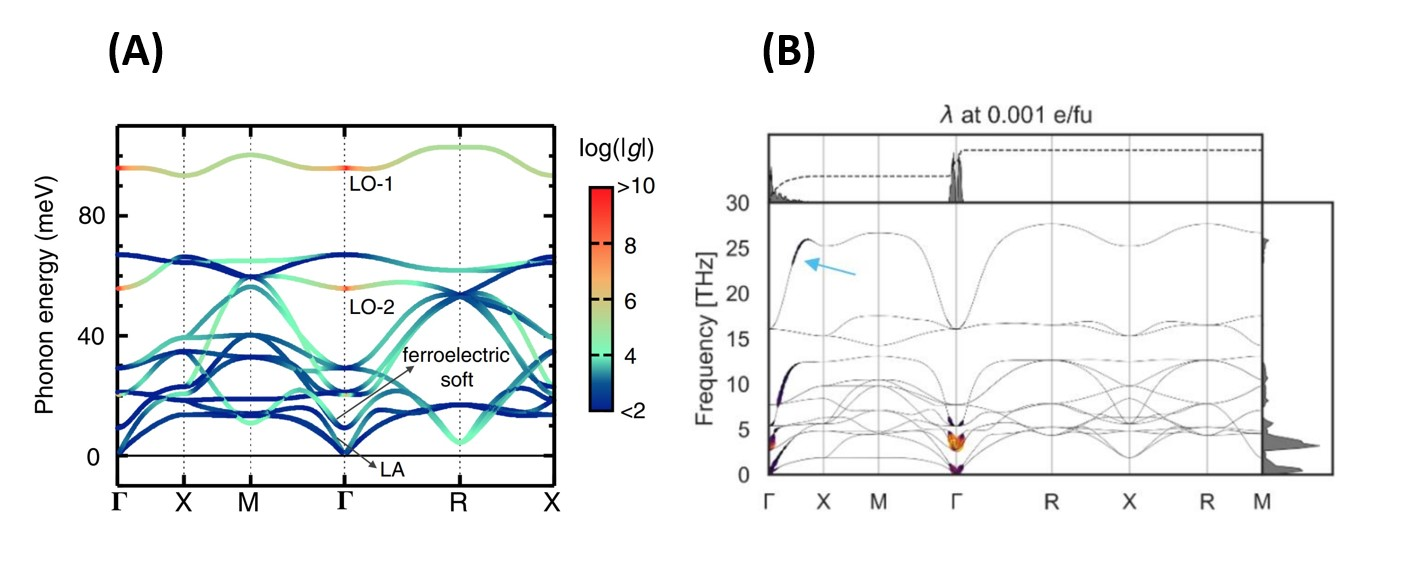
\includegraphics[width=0.8\textwidth]{figures/new_second_figure.jpg}
    \caption{\textbf{(A)} and \textbf{(B)}: Theoretically calculated EPC in $\mathrm{SrTiO_3}$ and $\mathrm{KTaO_3}$ respectively. Strong coupling of longitudinal optical mode (LO) can be seen near $\Gamma$ point. Blue arrow points at the LO mode in  $\mathrm{KTaO_3}$ (from Ref.\cite{zhou_electron-phonon_2018} and Ref.\cite{esswein_first-principles_2023} respectively).}  
\end{figure}
\paragraph{Project 2: Electron-phonon coupling in SrTiO$_{3}$ and KTaO$_{3}$} 
SrTiO$_{3}$ is a well-known superconducting material with a critical temperature of $\lesssim 1\, \mathrm{K}$\cite{schooley_superconductivity_1964,lin_fermi_2013}. 
Although it has a  relatively simple crystal structure, the mechanism of superconductivity in SrTiO$_{3}$ is still debated and probably unconventional. 
Among all the puzzles\footnote{These puzzles will be briefly discussed in the next section.}, the most intriguing are the extreme dilution of carriers and the reversed isotope effect: substitution of ${}^{16}\mathrm{O}$ by ${}^{18}\mathrm{O}$ surprisingly increases the critical temperature, contradicting the conventional BCS theory\cite{stucky_isotope_2016}. 
We propose investigating this effect by studying the EPC in SrTiO$_{3}$ using RIXS. If the reversed isotope effect is also seen in EPC, it would be strong evidence that EPC plays a role in SrTiO$_{3}$ superconductivity.

Another material of interest is KTaO$_{3}$, which, though not superconducting in bulk, exhibits superconductivity on $\mathrm{LaAlO_{3}/KTaO_{3}}$ (LAO/KTO) interface, reported recently in Ref.\cite{ren_two-dimensional_2022}. 
However, unlike LAO/SrTiO$_{3}$ interface where the superconductivity was found in all directions, the LAO/KTO interface exhibits a strong orientation-dependence of critical temperature\cite{ren_two-dimensional_2022,chen_two-dimensional_2021}. Similar to the hypothesis in SrTiO$_{3}$, the orientation-dependent superconductivity observed in LAO/KTO might be attributed to the anisotropic EPC. 
To deepen our understanding, we aim to quantitatively and experimentally measure the EPC in LAO/KTO in different direction. 

Therefore, we propose studying the isotope effect of the EPC in SrTiO$_{3}$, and the orientation dependence of EPC in LAO/KTO interface. 
Resonant inelastic X-ray scattering (RIXS) will be our main research tool. 
We expect to see a similar trend in EPC as in the superconducting critical temperature $T_{c}$, if the EPC does play a role in superconductivity in these materials.

% jump A
\paragraph{Project 3: Electron-phonon coupling in sapphire, a potential material for sub-MeV dark matter detection}
The concept of dark matter has long been shrouded in mystery in the field of modern physics. 
Despite numerous efforts to study and detect dark matter\cite{bergstrom_non-baryonic_2000,vogel_dark_2014,essig_first_2012,davidson_updated_2000}, the exact mass of the dark matter particle remains unknown. 
Various experimental tools have been utilized to cover a range of masses for dark matter detection. 
Phonon-based detector, for example, can be used to detect the sub-MeV dark matter (10 keV -- 1 MeV)\cite{griffin_directional_2018}.
  
In dark matter models, dark matter particles interact with phonons, in a similar manner to electrons\cite{griffin_directional_2018}. Therefore, measuring the EPC is essential for advancing dark matter detection. 
Recent studies have identified sapphire as a suitable material for phonon-based dark matter detection, attributed to its polar nature, anisotropy, and minimal screening effect\cite{griffin_directional_2018}.
Therefore, we propose conducting a RIXS study on sapphire to experimentally extract the EPC. Accurate measurements of this coupling are expected to significantly facilitate the detection of dark matter using sapphire.

All three projects are related to the measurement of EPC. This requires the use of RIXS and numerical simulation.

\begin{figure}[!t]
    \centering
    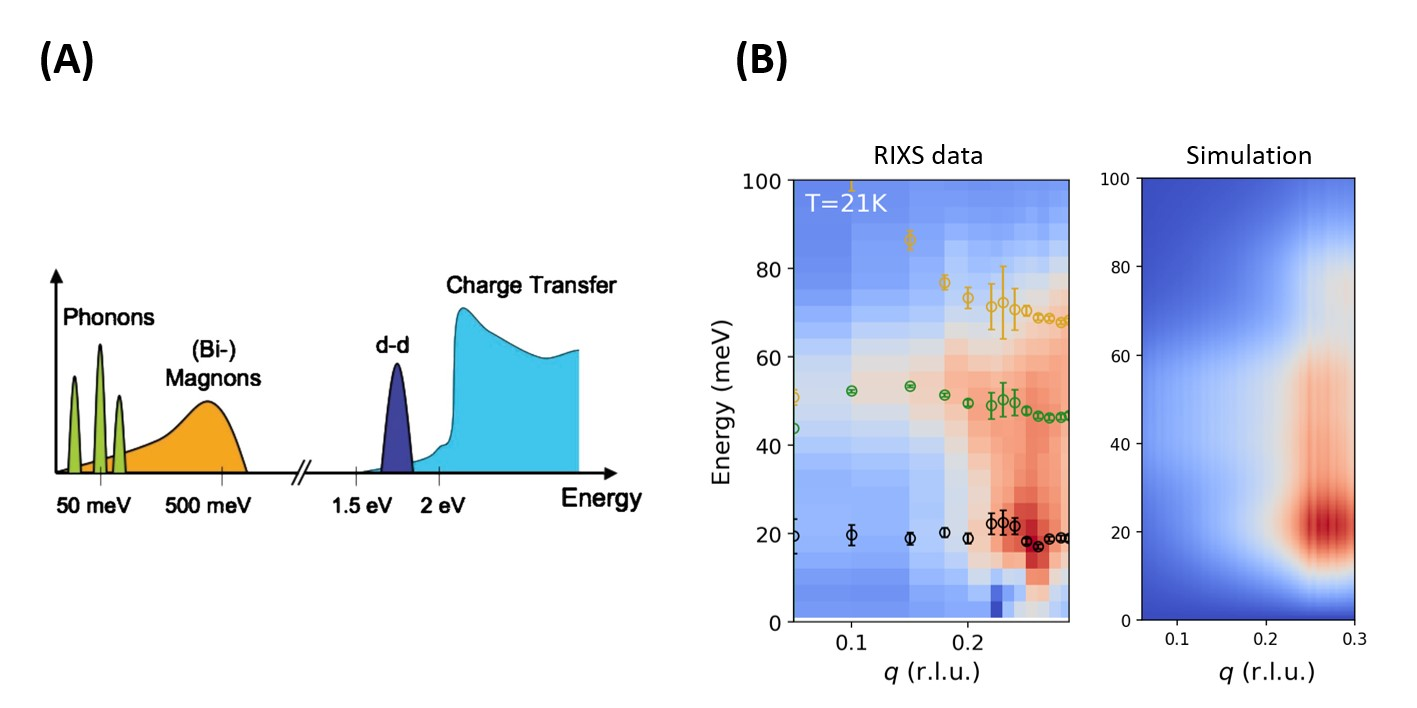
\includegraphics[width=0.8\textwidth]{figures/new_figure2.jpg}
    \caption{\textbf{(A)}: An illustration of possible excitations observed via RIXS. In the low-energy region there are phonons, which is our main focus in the projects (adapted from Ref.\cite{ament_resonant_2011}); \textbf{(B)}: A comparison between RIXS data and simulation outcomes. The left panel is the RIXS spectrum in project 1 (with elastic signal subtracted), with markers delineating the dispersions of three phonon branches; The right panel showcases the corresponding RIXS simulation conducted by myself.}  
    \label{simulation}
\end{figure}

\paragraph{Research method: resonant inelastic X-ray scattering (RIXS) and numerical simulation}
The extraction of EPC has historically been challenging in condensed matter physics. 
Before the advent of RIXS, conventional experimental methods, such as neutron scattering or ARPES, are not directly related to the EPC. 
RIXS, on the other hand, enables a more direct extraction of the EPC. 
The concept of probing the EPC using RIXS was first introduced by Ament et al. in 2011 \cite{ament_resonant_2011}. They proposed a model to describe the phonon intensity in RIXS, with simplification and approximation.
However, the energy resolution was at that time ($\sim100$ meV) still too low compared to phonon energies ($20-100$ meV). 
However, thanks to the recent advancement in RIXS\cite{zhou_i21_2022,brookes_the_2018}, the resolution at copper-$L_3$ edge and oxygen-$K$ edge can reach up to $\sim 35\,\mathrm{meV}$ and $\sim 20\,\mathrm{meV}$ respectively, making it possible to separate phonon signal from pure elastic signal. 
More sophisticated models were later proposed to describe the phonon intensity in RIXS using Feynman diagrams \cite{devereaux_directly_2016,matsubayashi_numerical_2023,bieniasz_theory_2022,geondzhian_generalization_2020} or density matrix renormalization group method\cite{nocera_computing_2018}, which allows us to \textit{simulate} the RIXS phonon response.

However, Ament's model requires localized electrons and dispersiveless phonons, which is a relatively stringent assumption for a vast majority of superconducting systems. 
Consequently, there is a pressing need for a theory beyond Ament's model to encompass a wider range of materials, and handle simulations in more complex scenarios. 
{During my research, I aim to venture into this unexplored field, trying to develop new theoretical frameworks and numerical tools for extraction of EPC in various superconducting materials.} 
Since my Master's research, I have been engaged in performing numerical simulation of RIXS spectra based on the diagrammatic method discussed in Ref.\cite{devereaux_directly_2016} (refer to Fig.\ref{simulation} for an illustrative simulation). 
Nonetheless, this method accounts only for single-phonon excitation process, while the theory for multi-phonon excitations remains missing.
According to Ament\cite{ament_determining_2011}, the inclusion of phonon overtones (i.e. multi-phonon excitations) is essential for determining the absolute value of EPC. 
\textit{This is the starting point of the simulation part of my research}: I intend to expand the diagrammatic method to encompass two-phonon excitations, thereby enabling a better extraction of EPC across a wider range of superconductors. 
Additional effort will also be dedicated to relaxing the assumptions presented in Ament's model.

% According to the theoretical models, phonon intensity in RIXS spectra is \textit{influenced} by the electron-phonon coupling\cite{devereaux_directly_2016}. In the case where electron-phonon coupling is independent of the momentum of the excited electron, the phonon intensity in the RIXS spectrum is \textit{directly proportional}  to the square of the electron-phonon coupling. Under the approximation that electron-phonon coupling is a constant, the \textit{relative} magnitude of the electron-phonon coupling can be calculated directly from the phonon intensity in the RIXS spectra. Additionally, the \textit{absolute} value of electron-phonon coupling can be further determined by either (1) comparing phonon intensity with its overtones; or (2) analyzing changes in phonon intensity upon detuning the incident energy\cite{ament_resonant_2011,braicovich_determining_2020}. Further development in RIXS theory proposes modification in Ament's model, accounting for the momentum dependence of electron-phonon coupling and relaxing some of its stringent assumptions in Ament's model\cite{bieniasz_theory_2022,geondzhian_generalization_2020}. 

%Despite all that, RIXS is still considered the best tool for our projects due to its strong power in measuring phonons and the potential to EPC. Thanks to the recent development in RIXS, the resolution at copper-L edge and oxygen-K edge can reach up to $\sim 35\,\mathrm{meV}$ and $\sim 20\,\mathrm{meV}$ respectively, making it possible to separate phonon signal from pure elastic signal. 
% Here we briefly summarize the use of RIXS in the three projects:
%\begin{itemize}
%  \item In project 1 (cuprate superconductor project), both charge order and phonons can be observed by RIXS. By simulating phonon and charge order spectrum separately, we can study the interplay between phonons and charge order. 
%  \item In project 2 (STO and KTO project) and project 3 (sapphire project), the use of RIXS is more straightforward: acquiring the RIXS spectrum and directly extracting the electron-phonon coupling using Ament's model.
%\end{itemize}



\section{Background Information and Current State of Research}
% \textit{\textbf{Instructions}: Describe your project in the context of the {\color{cyan}current state of research} in your field. Refer to the most important publications, especially by other authors. {\color{cyan}Describe which previous findings are the starting point and basis for the planned studies}, where and why there is a need for research and which important, relevant research is currently underway in Switzerland and abroad. } 

The first superconductor was discovered in mercury (Hg) in 1911 by Kamerlingh Onnes. Since then, superconductivity has been observed in many materials, and the mechanism of superconductivity had been studied extensively.
In 1957, Bardeen, Cooper, and Schrieffer introduced the BCS theory, the first successful theoretical framework to explain superconductivity\cite{bardeen_theory_1957}. 
In BCS theory, 
%phonons are believed to mediate the superconductivity. 
%More specifically, 
the interaction between phonons and electrons (the electron-phonon coupling, EPC) fosters an effective attractive force among electrons, leading to the formation of Cooper pairs and driving the superconducting transition~\cite{bardeen_theory_1957}. 
In 1986, Bednorz and Müller discovered a lanthanum-based (La-based) cuprate material that became superconducting at a striking $35\,\mathrm{K}$\cite{bednorz_possible_1986}, heralding a new era of high-temperature superconductors. 
%Since then, many  high-temperature superconductors have been discovered, including $\mathrm{YBa_{2}Cu_{3}O_{7-x}}$\cite{wu_superconductivity_1987}, $\mathrm{Bi_2Sr_2CaCu_{2}O_{8+x}}$\cite{maeda_a_1988}, and more. 
However, BCS theory falls short in explaining this type of superconductivity, with its underlying mechanism still being a subject of intense debate \cite{keimer_quantum_2015}.
%Many new theories have been put forward, attempting to explain the superconducting phenomenon at high temperature.
Nonetheless, even if BCS theory is not able to explain the mechanism, the concept of phonon-mediated interactions is still believed to play a role in high-temperature superconductivity. 
There are several reasons: \textbf{(1)} It's theorized that phonons, along with other pairing-driving excitations, could enhance superconducting critical temperature\cite{johnston_systematic_2010}, and an interesting relation between the superconducting gap and the EPC with specific oxygen vibrations was recently observed \cite{he_rapid_2018}; 
additionally, \textbf{(2)} the coherent, ultrafast excitations of an apical oxygen phonon mode in some cuprate materials appears to facilitate superconductivity~\cite{kaiser_optically_2014};
furthermore, 
%\textbf{(3)} charge order in cuprate is assumed to compete with the superconducting phase, while phonon was observed to interact with both static and dynamical charge order\cite{arpaia_charge_2021,comin_resonant_2016,canosa_resonant_2014, hucker_competing_2014, chang_direct_2012,ghiringhelli_long-range_2012,wang_charge_2021,lin_strongly_2020, huang_quantum_2021,miao_incommensurate_2018,tacon_inelastic_2014,li_multiorbital_2020,braicovich_determining_2020,chaix_dispersive_2017,peng_enhanced_2020}. 
\textbf{(3)} many experiments have shown that phonons are deeply intertwined with charge order, which is universally present in cuprates superconductors \cite{arpaia_charge_2021,comin_resonant_2016,canosa_resonant_2014, hucker_competing_2014, chang_direct_2012,ghiringhelli_long-range_2012,wang_charge_2021,lin_strongly_2020, huang_quantum_2021,miao_incommensurate_2018,tacon_inelastic_2014,li_multiorbital_2020,braicovich_determining_2020,chaix_dispersive_2017,peng_enhanced_2020}. 
%Therefore, a better understanding of phonon, especially its interaction with electron and electronic orders, will certainly shed light on the mechanism of superconductivity.  

%The first part of this project is based on the third point mentioned above. 
%Charge order
%,a universal phenomenon in various families of cuprate superconductors, exhibits a distinct interplay with superconducting phase.
%In La-based cuprate is believed to stem from a strong electronic interactions which results in a so-called stripe order\cite{harriger_stripe_nodate,tranquada_evidence_1995,choi_disentangling_2020}. 
%This stripe order, different from the usual charge order, is likely not induced by special features in momentum-dependent electron-phonon coupling. 
Indeed, several anomalies in the phonon response have been observed in the vicinity to the charge order vector.
%indicates a possible interaction between phonon and both static and dynamical charge order.
%
%\begin{itemize}
%\item \textit{Phonon softening}  was observed near the charge order wavevector In $\mathrm{La_{2-x}Sr_{x}CuO_{4}}$\cite{lin_strongly_2020, wang_charge_2021, huang_quantum_2021}, $\mathrm{La_{2-x}Ba_{x}CuO_{4}}$\cite{miao_incommensurate_2018}, $\mathrm{YBa_{2}Cu_{3}O_{6+x}}$\cite{tacon_inelastic_2014}, $\mathrm{Bi_{2}Sr_{2}LaCuO_{6+\delta}}$\cite{li_multiorbital_2020}, and other families. 
%The root cause of this phenomenon is not clear, as many factors could contribute to the phonon softening, such as pure lattice distortions~\cite{lin_strongly_2020}, and interactions between phonon and other excitations.  
%\item \textit{Enhancement in phonon intensity}  in RIXS measurement was observed in $\mathrm{Bi_{2}Sr_{2}LaCuO_{6+\delta}}$\cite{li_multiorbital_2020}, $\mathrm{Bi_{2}Sr_{2}CaCu_{2}O_{8+\delta}}$\cite{chaix_dispersive_2017}, $\mathrm{Nd_{1+x}Ba_{2-x}Cu_{3}O_{7+\delta}}$\cite{braicovich_determining_2020}, and {La$_{1.8-x}$Eu$_{0.2}$Sr$_x$CuO$_{4}$}\cite{peng_enhanced_2020,wang_charge_2021,huang_quantum_2021}. 
%However, it was also reported that phonon intensity in $\mathrm{La_{2-x}Sr_{x}CuO_{4}}$ remains relatively unchanged across a wide range of doping, even when charge order disappears\cite{lin_strongly_2020}.  
%\end{itemize}
%
A softening in the energy of bond-stretching oxagen modes was observed near the charge order wavevector in $\mathrm{La_{2-x}Sr_{x}CuO_{4}}$\cite{lin_strongly_2020, wang_charge_2021, huang_quantum_2021}, $\mathrm{La_{2-x}Ba_{x}CuO_{4}}$\cite{miao_incommensurate_2018}, $\mathrm{YBa_{2}Cu_{3}O_{6+x}}$\cite{tacon_inelastic_2014}, $\mathrm{Bi_{2}Sr_{2}LaCuO_{6+\delta}}$\cite{li_multiorbital_2020}, and other families. 
The root cause of this phenomenon is not clear, as many factors could contribute to the phonon softening, such as pure lattice distortions~\cite{lin_strongly_2020}, and interactions between phonon and other excitations.  
At the same time an enhancement of phonon intensity in RIXS measurements was observed in $\mathrm{Bi_{2}Sr_{2}LaCuO_{6+\delta}}$\cite{li_multiorbital_2020}, $\mathrm{Bi_{2}Sr_{2}CaCu_{2}O_{8+\delta}}$\cite{chaix_dispersive_2017}, $\mathrm{Nd_{1+x}Ba_{2-x}Cu_{3}O_{7+\delta}}$\cite{braicovich_determining_2020}, and {La$_{1.8-x}$Eu$_{0.2}$Sr$_x$CuO$_{4}$}\cite{peng_enhanced_2020,wang_charge_2021,huang_quantum_2021}. 
However, it was also reported that phonon intensity in $\mathrm{La_{2-x}Sr_{x}CuO_{4}}$ remains relatively unchanged across a wide range of doping, even when charge order disappears\cite{lin_strongly_2020}.  
Interestingly, a recent experiment performed by Johan Chang's quantum matter research group at the University of Zurich, in which I participated, brought results in contradiction with some of these interpretations. 
Uniaxial pressure was applied to modulate the intensity of charge order in $\mathrm{La_{2-x}Sr_{x}CuO_{4}}$ differently along the two in-plane directions. 
It was found that phonon intensities and energies remain unchanged regardless of the suppression or enhancement of the quasi-static charge order intensity. 
This findings implies a potential decoupling between phonon and charge order excitations in $\mathrm{La_{2-x}Sr_{x}CuO_{4}}$, supporting the theory given in Ref.\cite{lin_strongly_2020}, but contradicting some other studies\cite{li_multiorbital_2020, chaix_dispersive_2017,huang_quantum_2021}. 

Due to the nature of RIXS, an enhancement in phonon intensity could stem from different factors: \textbf{(1)} an increase in the EPC into the charge order phase as proposed in Ref.\cite{wang_charge_2021,peng_electronic_2022}; 
or \textbf{(2)} interaction between phonon and charge order excitations as discussed in Ref.\cite{li_multiorbital_2020, chaix_dispersive_2017,huang_quantum_2021}; 
or \textbf{(3)} extra excitations overlapping with phonon, creating extra RIXS signals on top of phonon spectrum, which has long been considered as part of the phonon spectrum itself. 
%\textit{It is important to note that point (3) is the starting point of my first project.} 
The first part of my PhD project will be devoted to the investigation of this effects.
We hypothesize that the enhancement in phonon intensity in cuprate is due to charge excitation signals overlapping with the phonon signal, rather than direct interaction with phonon itself.  
We seek to explore the nature of charge order excitations in {La$_{1.8-x}$Eu$_{0.2}$Sr$_x$CuO$_{4}$} with RIXS under this hypothesis, and furthermore extend our model to other cuprate materials. 
Through this study, we aim to offer a novel insight into the relation between phonon and charge order excitations in cuprate superconductors. 
To achieve this, we plan to utilize RIXS for conducting measurements on {La$_{1.8-x}$Eu$_{0.2}$Sr$_x$CuO$_{4}$}, followed by simulating the RIXS spectrum based on the model proposed in Ref.\cite{devereaux_directly_2016}. 
By comparing simulation and experimental results, we will gain a deeper understanding of the charge order excitations' properties in this material. 
Further development of numerical technique is also ongoing, and a more accurate simulation of RIXS spectrum in this material can be foreseen.

Beyond cuprates, the EPC also plays a pivotal role in other unconventional superconductors. 
SrTiO$_{3}$ is a fascinating example. It is considered a very ``dilute'' superconductor, exhibiting
superconductivity even with charge carrier densities as low as $\sim 10^{17}\,\mathrm{cm^{-3}}$\cite{schooley_superconductivity_1964,lin_fermi_2013}, a characteristic shared with other systems like $\mathrm{Pb_{1-x}Tl_{x}Te}$\cite{known} and single crystal $\mathrm{Bi}$\cite{prakash_evidence_2017}. 
%Theoretical studies suggested that in SrTiO$_{3}$, phonon-mediated interactions are instrumental in driving superconductivity, notably causing an increase in superconducting transition temperature as the material becomes more electron-dilute\cite{gastiasoro_phonon-mediated_2019}.
Investigation into SrTiO$_{3}$ revealed a polaronic behavior, where the electronic energy band is significantly renormalized by the interaction with high-energy longitudinal optical phonons \cite{swartz_polaronic_2018, geondzhian_large_2020}.
Given the strong EPC that is at the base of polaron formation, these longitudinal optical branches are, as suggested by some studies\cite{gastiasoro_supercondutivity_2020}, possibly involved in driving superconductivity in SrTiO$_{3}$.
However, such a conventional electron-phonon interaction cannot explain the superconducting behavior in SrTiO$_{3}$: 
\textbf{(1)} BCS theory requires a higher Fermi energy compared to the phonon energy, which is not satisfied in this system;
\textbf{(2)} Despite strong interactions between longitudinal optical phonons and electrons, the relatively small superconducting gap suggests a weak effective EPC, diverging from conventional superconductor behavior\cite{swartz_polaronic_2018}; 
\textbf{(3)} A reverse isotope effect has been observed: the superconducting critical temperature increases by $50\%$  when $35\%$ of the ${}^{16}\mathrm{O}$ is replaced with ${}^{18}\mathrm{O}$\cite{stucky_isotope_2016}, again contradicting predictions of conventional theory. Interestingly, such substitution also drives the system in a ferroelectric phase\cite{stucky_isotope_2016}.
%According to the first point, even though there's a discrepancy between the actual electron-phonon coupling and the required coupling for superconductivity, it's still unknown whether this phonon branch contributes to inducing superconductivity.
Alternative theories have been developed to explain the emergence of superconductivity in SrTiO$_{3}$. Among them, the most discussed is the possibility that superconductivity is mediated by ferroelectric fluctuations. In particular, the transverse optical phonons with low-energy that drive the ferroelectric transition could mediate Cooper pairing \cite{gastiasoro_supercondutivity_2020}. The difficulty of such model is that the standard EPC (e.g. the Froehlich interaction) of transverse phonons is extremely small, so that the coupling to electron should be mediated by more exotic bi-phonon interactions \cite{gastiasoro_phonon-mediated_2019}.
Therefore, at present it is still not known whether superconductivity is mainly induced by high-energy, longitudinal phonon modes or by low-energy transverse branches.
\textit{To shed light on this topic, we propose studying the reverse isotope effect to address these discrepancies.} We plan to conduct a RIXS measurement on SrTiO$_{3}$ with varying oxygen isotope compositions to investigate how EPC varies with the substitution ratio.  Should longitudinal optical phonons contribute to superconductivity, we anticipate observing a similar trend in EPC as in the superconducting transition temperature $T_{c}$. If this is the case, both questions mentioned above will be much clearer to us. 

Another material, KTaO$_{3}$ with a similar crystal structure to SrTiO$_{3}$, has recently been discovered to host superconductivity on the surface\cite{ren_two-dimensional_2022}. 
Contrasting with SrTiO$_{3}$, \textit{bulk}  electron-doped KTaO$_{3}$ is not superconducting, yet superconductivity emerges at the $\mathrm{LaAlO_{3}/KTaO_{3}}$ interface\cite{ren_two-dimensional_2022,chen_two-dimensional_2021}. 
Notably, the superconducting critical temperature $T_c$ at the $\mathrm{LaAlO_{3}/KTaO_{3}}$ interface shows a strong orientation dependence\cite{ren_two-dimensional_2022,chen_two-dimensional_2021}. 
More specifically: 
\textbf{(1)} For the $(111)$ orientation, $T_{c} = 2\,\mathrm{K}$\cite{ren_two-dimensional_2022};
\textbf{(2)} In $(110)$ direction, $T_{c} = 0.9\,\mathrm{K}$\cite{chen_two-dimensional_2021};
\textbf{(3)} However, in $(001)$ direction, no superconducting phase has been detected even at temperature as low as $25\,\mathrm{mK}$\cite{ren_two-dimensional_2022}. 
Similar to SrTiO$_{3}$\cite{swartz_polaronic_2018}, polaronic behavior has also been observed in KTaO$_{3}$, again suggesting a strong interaction between electron and longitudinal optical phonon\cite{chen_orientation-dependent_2023}. 
It is possible that phonon-mediated interaction also plays a part in driving superconductivity in KTaO$_{3}$. 
\textit{Therefore, to investigate this phenomenon, we propose to perform RIXS measurements on KTaO$_{3}$ in various orientations, and extracting the EPC.}
Our expectation is that the trends observed in EPC will mirror the trends seen in the superconducting critical temperature $T_c$. 

%In both SrTiO$_{3}$ and KTaO$_{3}$, our primary focus lies on the investigation of EPC. 
%Thanks to the powerful tool of RIXS, it is possible to extract the absolute values of the momentum-dependent electron-phonon coupling directly. 
%Naturally, this relies on the advancement of numerical technique for RIXS simulation, an area in which I am involved and making advancements.
% jump B
Furthermore, the importance of EPC extends beyond superconductivity, playing a crucial role in other cutting-edge research areas like dark matter detection. The detection of dark matter is one of the most important problems in physics, as it is one of the two famous unsolved problems in modern physics, together with dark energy.
The concept of dark matter, first proposed by Zwicky in 1933\cite{andernach_english_2017}, was introduced to explain the anomalously high gravitational forces in galaxies, which exceed those expected from ordinary observable mass alone. However, the direct detection of dark matter has so far been unsuccessful,
%due to the weak interaction between dark matter and ordinary matter.
Various methods have been developed to detect dark matter\cite{bergstrom_non-baryonic_2000}, each of which covers a different range of the dark matter mass\cite{vogel_dark_2014,essig_first_2012,davidson_updated_2000}. Among these, phonon-based detection stands out for its potential in detecting sub-MeV dark matter (ranging from $ 10\,\mathrm{keV}$ -- $1\,\mathrm{MeV}$). This method hinges on the interaction between dark matter particles and phonons, akin to the interaction between electrons and phonons\cite{griffin_directional_2018}. 

\begin{figure}
    \centering
    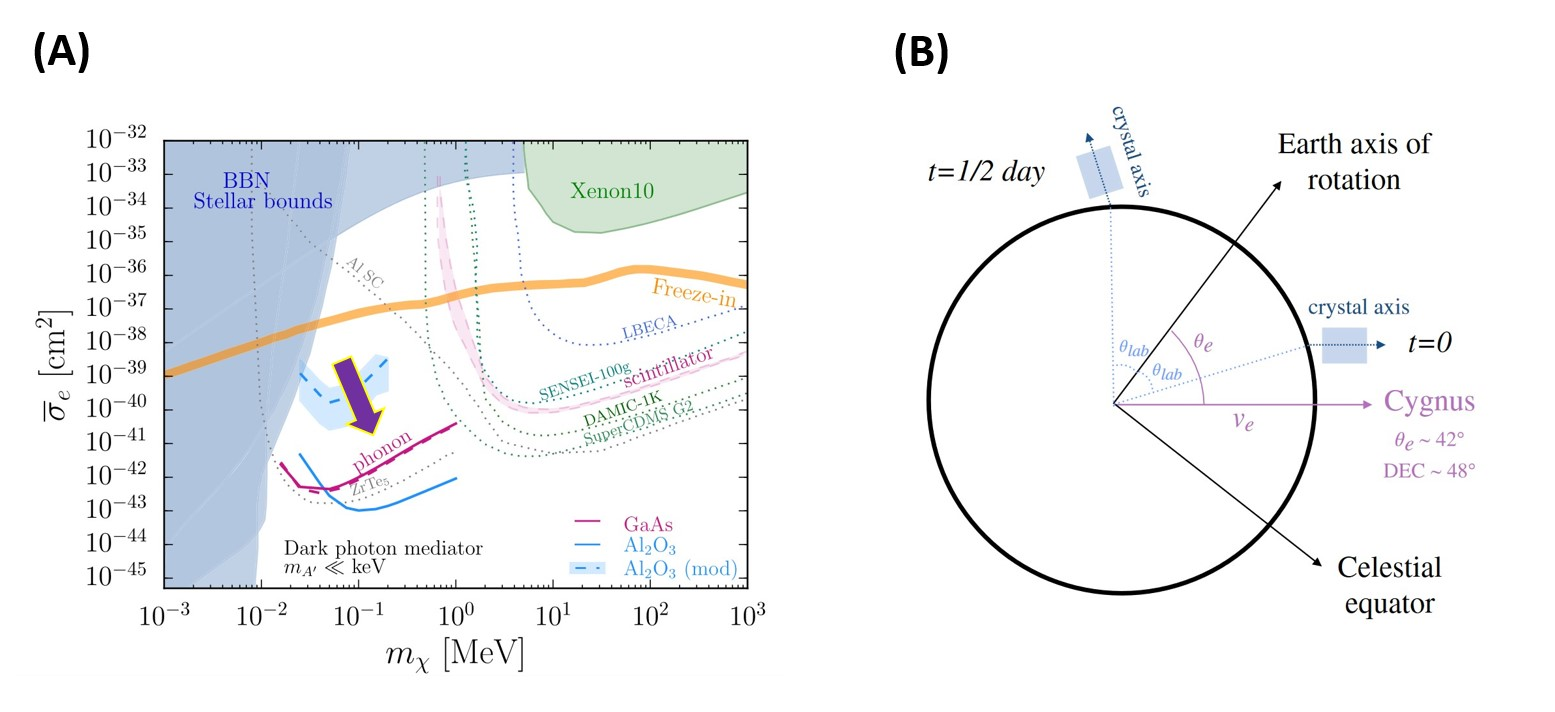
\includegraphics[width=0.9\textwidth]{figures/third_figure.jpg}
    \caption{\textbf{(A)} Cross section of phonon-based dark matter detection, pointed at by purple arrow, along side with other detection techniques (from Ref.\cite{griffin_directional_2018}); \textbf{(B)} An illustration of daily-modulated dark matter signal. The dark matter flux goes through the crystal in different direction at a different time of a day (from Ref.\cite{griffin_directional_2018}).}
    \label{third_figure}
\end{figure}



Recently, a new material, sapphire, has been proposed as suitable material for phonon-based dark matter detection\cite{griffin_directional_2018}. According to this study, sapphire's suitability for phonon-based dark matter detection stems from several factors: 
\textbf{(1)} As a polar material, sapphire is  expected to interact strongly with dark matter, aided by dark photon mediation; 
\textbf{(2)} Its insulating nature results in minimal screening effects, potentially enhancing phonon-dark matter interactions; 
\textbf{(3)} Sapphire's anisotropic property allows for the discrimination of dark matter particles from other types of particles. 
The anisotropy implies that both electron-phonon coupling and dark-matter-phonon coupling are direction-dependent\cite{griffin_directional_2018}, leading to an anisotropic cross section for dark matter detection. 
Due to the Earth's rotation, the dark matter signal is expected to vary throughout the day as the direction of dark matter flux changes, depending on the orientation of the Earth. 
This daily-modulated property enables us to distinguish dark matter signal from other background noise.
The first step towards detecting sub-MeV dark matter is to measure the EPC in sapphire, on the assumption that this coupling mirrors the dark-matter-phonon interaction. 
\textit{Therefore, we propose conducting a RIXS measurement on sapphire to extract the EPC in different orientation.}  
We expect to observe an anisotropic behavior in the phonon signal in RIXS spectrum. 
Afterwards, we will carefully extract the EPC based on Ament model\cite{ament_determining_2011}. 
This investigation represents a foundational step in our journey towards dark matter detection.

In project (2) and (3) on SrTiO$_{3}$ KTaO$_{3}$ and sapphire, our primary focus lies on the investigation of EPC. 
Thanks to the powerful tool of RIXS, it is possible to extract the absolute values of the momentum-dependent EPC directly. 
{However, this goal relies on the advancement of numerical modelling of the RIXS cross section. At present, no rigorous simulation of the RIXS phonon response in insulating oxides has been performed. I will contribute to this aim. In particular, my goal is to apply and expand the diagrammatic approach to the RIXS cross section that has been used to simulate the spectra of cuprates \cite{devereaux_directly_2016}. This approach has already been used in my Master's thesis project. }

\section{Planned Research Activities and Schedule}
\begin{center}
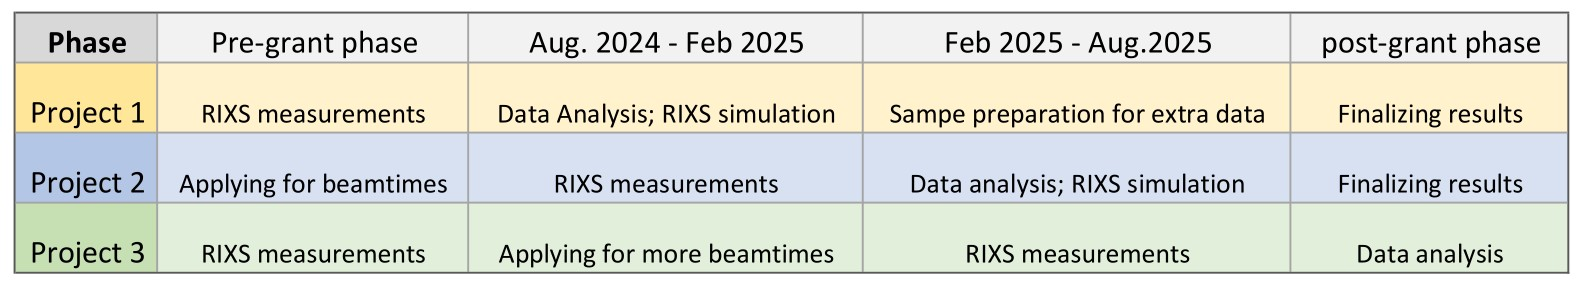
\includegraphics[width=0.99\textwidth]{figures/schedule.jpg}
\end{center}
\paragraph{Project 1: Charge and Lattice Dynamics in Cuprate Superconductors}
We have completed the initial experimental phase of the first project, which involved RIXS measurements on {La$_{1.8-x}$Eu$_{0.2}$Sr$_x$CuO$_{4}$} (with $x=0.125$) at Diamond Light Source's I21 beamline in the UK. More experiment might be needed due to the lack of data of {La$_{1.8-x}$Eu$_{0.2}$Sr$_x$CuO$_{4}$} with different doping levels. We plan to apply for beamtime at I21 again in the next application cycle. Detailed schedule is as follows
\begin{itemize}
  \item \textit{Pre-grant phase}: Collecting RIXS data of $\mathrm{La_{1.675}Eu_{0.2}Sr_{0.125}CuO_{4}}$ at oxygen-K edge at beamline I21 at Diamond Light Source, focusing primarily on the temperature dependence of charge order and phonon. 
  \item \textit{First phase, Aug.2024 -- Feb.2025}: Analyzing data to extract EPC, simulating charge order and phonon spectrum, and characterizing charge order excitations. In the meantime, we will apply for additional beamtime for further RIXS experiments on {La$_{1.8-x}$Eu$_{0.2}$Sr$_x$CuO$_{4}$} with different doping levels. 
  \item \textit{Second phase, Feb.2025 -- Aug.2025}: Preparing {La$_{1.8-x}$Eu$_{0.2}$Sr$_x$CuO$_{4}$} samples with different doping for subsequent RIXS experiments. 
  \item \textit{Post-grant phase}: Concluding,  finalizing results and drafting the manuscript for publication.
\end{itemize}

\paragraph{Project 2: Electron-Phonon Coupling in SrTiO$_{3}$ and KTaO$_{3}$}
The proposal of SrTiO$_{3}$ has been submitted to beamline I21 at Diamond Light Source, and was accepted earlier by the time of this application. The date of the beamtime has not been scheduled yet, but it is most likely to be in 2024. The proposal of KTaO$_{3}$ has been submitted to beamline 41A at Taiwan Photon Source in Taiwan. 
\begin{itemize}
  \item \textit{Pre-grant phase}: Applying for a beamtime at I21 (Diamond Light Source) and 41A (Taiwan Photon Source).
  \item \textit{First phase, Aug.2024 -- Feb.2025}: Preparing Samples and conducting RIXS experiment on SrTiO$_{3}$ at I21 and KTaO$_{3}$ at 41A. 
  \item \textit{Second phase, Feb.2025 -- Aug.2025}: Data analysis, extracting EPC in both SrTiO$_{3}$ and KTaO$_{3}$. Examining the reverse isotope effect and the possible anisotropy of the electron phonon interaction.
  \item \textit{Post-grant phase}:  Concluding,  finalizing results and preparing the manuscript for publication.
\end{itemize}

\paragraph{Project 3: Sub-MeV Dark Matter Detection}
The initial experiment on sapphire has been conducted at beamline 41A of Taiwan Photon Source in Taiwan ealier by the time of this application. However, more experiments are needed due to the lack of data in other directions and high-resolution data for (001) orientation. We intend to apply for additional beamtime at beamline ID32 of ESRF in France in the upcoming application cycle.
\begin{itemize}
  \item \textit{Pre-grant phase}: Performing initial experiment at beamline 41A, focusing on sapphire orientations $(0001)$, $(1\bar{1}02)$, and $(100)$. 
  \item \textit{First phase, Aug.2024 -- Feb.2025}: Applying for beamtime. Preparing Samples with orientation $(1\bar{1}00)$, $(21\bar{1}0)$, and $(100)$. 
  \item \textit{Second phase, Feb.2025 -- Aug.2025}: Conducting RIXS measurements on the prepared sapphire samples: $(1\bar{1}00)$, $(21\bar{1}0)$, and $(100)$. 
  \item \textit{Post-grant phase}: Data analysis, extracting EPC of all orientations we examined in sapphire.
\end{itemize}

\section{Available Resources}
All three projects require the use of RIXS instruments and high-quality samples. Access to synchrotron facilities and RIXS instruments hinges on successful approval of corresponding research proposals. The proposals are presented in two cycles annually. Our group, led by Prof. Johan Chang, is known for the high success rate (60-70\%) in securing RIXS proposals, bolstering our confidence in accessing these crucial resources. No major difficulties in getting access to beamtime are therefore foreseen. 

Samples are obtained from different sources: \textbf{(1)} High-quality {La$_{1.8-x}$Eu$_{0.2}$Sr$_x$CuO$_{4}$} (LESCO) samples are provided by Prof. Tohru Kurosawa from Muroran Institute of Technology, with whom we have long-standing collaboration. The samples obtained from him have already been used in multiple studies\cite{choi2022unveiling,wang_charge_2021} in Prof. Chang's group.
We also have the required expertise to precise polishing and cleaving the LESCO samples. Additionally, we have access to a SQUID magnetometer for magnetic susceptibility measurements and a Physical Property Measurement System (PPMS) for resistivity assessments.
\textbf{(2)} High-quality SrTiO$_{3}$ (STO) and KTaO$_{3}$ (KTO) samples are commercially available. we will collaborate with Dr. Benoît Fauqué from Collège de France, a renowned expert in oxide materials. His team will assist in characterizing these samples.
\textbf{(3)} High-quality, single-crystal, well-polished sapphire samples are also commercially available. We have the flexibility to procure these from various manufacturers (e.g. from Crystal GmbH).
In our labs, samples can be well characterized and finely aligned using Laue diffraction.

For numerical computations, our primary tool is a standard laptop, sufficient for most simulations. For more demanding computational tasks, we have access to the University of Zurich's science cluster\footnote{https://www.zi.uzh.ch/en/teaching-and-research/science-it/computing/sciencecluster.html}, which boasts high-performance GPUs and CPUs. Moreover, the machine learning project carried out in Prof. Johan Chang's group at University of Zurich will greatly facilitate the experiment measurement and the data analysis. RIXS's  effectiveness is significantly hampered by the lengthy duration of data acquisition and the relatively short allocation of beamtime. This machine learning project provides a way to denoise the RIXS data, and thus will be very helpful in accelerating the data acquisition process.  


\section{Significance of Expected Results}
\paragraph{Revealing the Nature of Charge Order Excitations in Cuprate Superconductors} While extensive research has been conducted on static charge order in cuprate, the dynamical charge order (or charge order excitations) are not fully understood. The interaction between phonons and charge order exictations remains an open question. Our study, in conjunction with another ongoing project on La$_{2-x}$Sr$_x$CuO$_4$ within our group, aims to answer this question. Moreover, our RIXS simulations will determine crucial parameters of charge order excitations, including the inverse lifetime, energy gap, and how these parameters evolve with temperature. This information is essential for the understanding of charge order excitations, especially away from the quantum critical point. 

\paragraph{Advancing Understanding in High-Temperature Superconductivity}
The investigation of EPC in SrTiO$_{3}$ and KTaO$_{3}$ is fundamental to unravel the mysteries of unconventional superconductivity.  We expected the trends in EPC to mirror those in the superconducting critical temperature. Should this hypothesis hold, it would suggest that the longitudinal optical phonons are part of the driving forces of superconductivity in both systems. We anticipate contributions to the understanding of the role played by EPC in unconventional superconductivity, potentially leading to new theoretical frameworks. 

\paragraph{Contributions to Dark Matter Research}
Our investigation into the EPC in sapphire represents a pioneering effort in the search for dark matter. By carefully characterizing electron-phonon interaction, and potentially dark-matter-phonon couplings, this project could significantly impact the design and sensitivity of future phonon-based dark matter detection experiments. 
This is undoubtedly the first step towards unmasking one of the most important problems in modern physics.

\paragraph{Methodological Advancements}
We aim to make use of RIXS not only experimentally, but also computationally and theoretically. Although RIXS is the best tool for the extraction of EPC, its power is currently highly limited by the lack of theories encompassing more superconducting systems and those describing multi-phonon excitation process. Rigorous numerical simulation technique is also needed. I expect to contribute to extending the theoretical framework to two-phonon excitation process and relaxing the stringent approximation made in Ament's model\cite{ament_resonant_2011}, as well as to developing numerical technique for oxygen-K edge simulation. This will enable a more accurate extraction of EPC in a wider range of quantum systems. 



\newpage
\bibliographystyle{unsrt}
\bibliography{ref}
%\addcontentsline{toc}{chapter}{References}

\end{document}
